\documentclass[12pt]{article}
\usepackage{fullpage}
\usepackage{graphicx}
\usepackage{xcolor}
\definecolor{TSIBlack}{HTML}{040404}
\begin{document}
\pagecolor{TSIBlack}
\color{white}
\tableofcontents
\begin{titlepage}
\begin{center}
\huge GAME MACHINE
\end{center}
\begin{center}
 BY
\end{center}
\begin{center}
\huge Tiny Shark Interactive
\end{center}
\begin{center}

\includegraphics[scale=0.6]{banner.png}
\end{center}
\end{titlepage}
\section{Introduction}
This Game Machine is a plugin for unreal engine 4.10 and above.
We have designed this plugin for designing mission.
\section{General description}
\section{Specific requirements}
\section{Overview}
\section{How to use}
	  \subsection{overview}
	  In game machine there are two type of graphs mission graph and dialogue graph which will going to give help mission designers to design missions easy and more afficent way.   
	  \subsection{MissionGraph}
	  Mission Graph is the place where we are going to define the flow of our mission and design objectives.
	  Here in mission graph there are four node's Mission-Root-Node, Objective-Node,Branched-Objective-Node,Multi-Objective-Node
	  \begin{center}
	  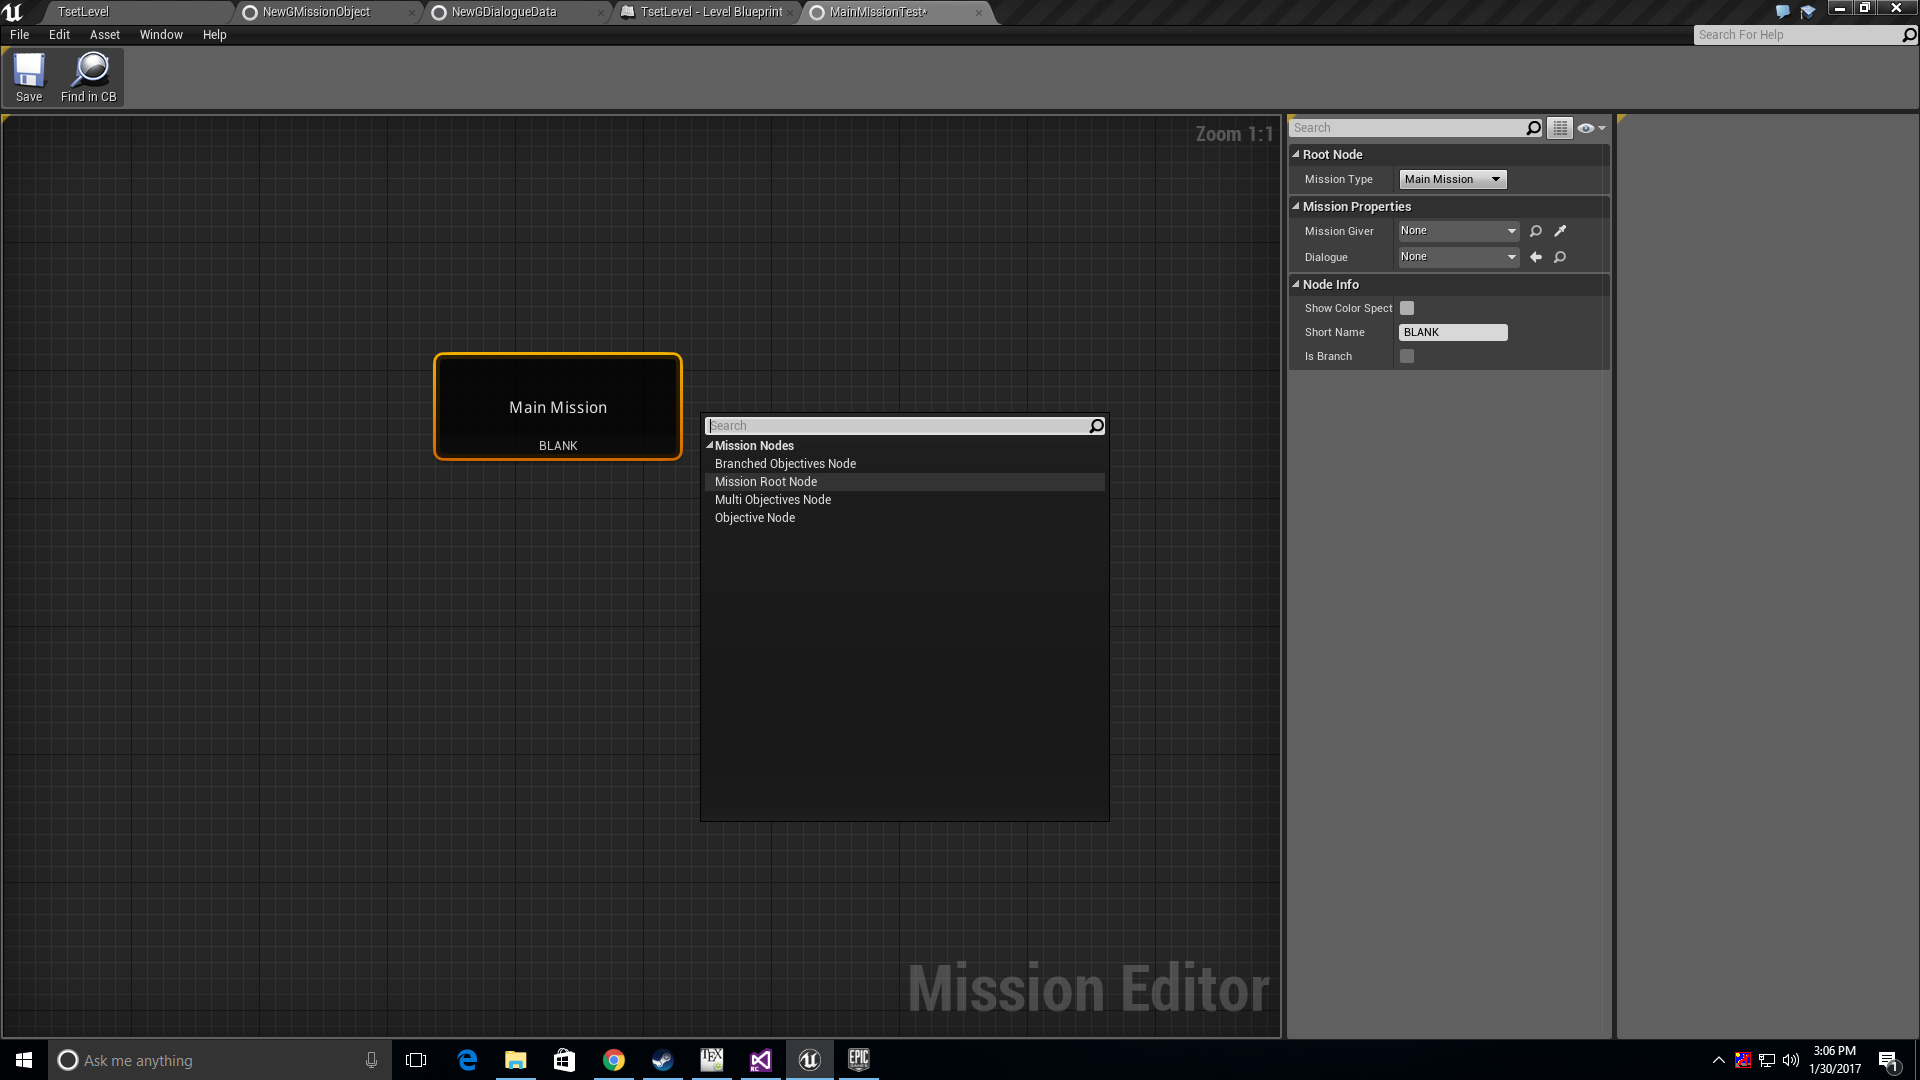
\includegraphics[scale=0.2]{MissionRootNode.png}
	  \end{center}
	  \begin{center}
	  \textit{MISSION ROOT NODE}\\
	  --------------------------------------
	  \end{center}
	  This is the entry node from where our mission will be initialized.
	  \begin{center}
	  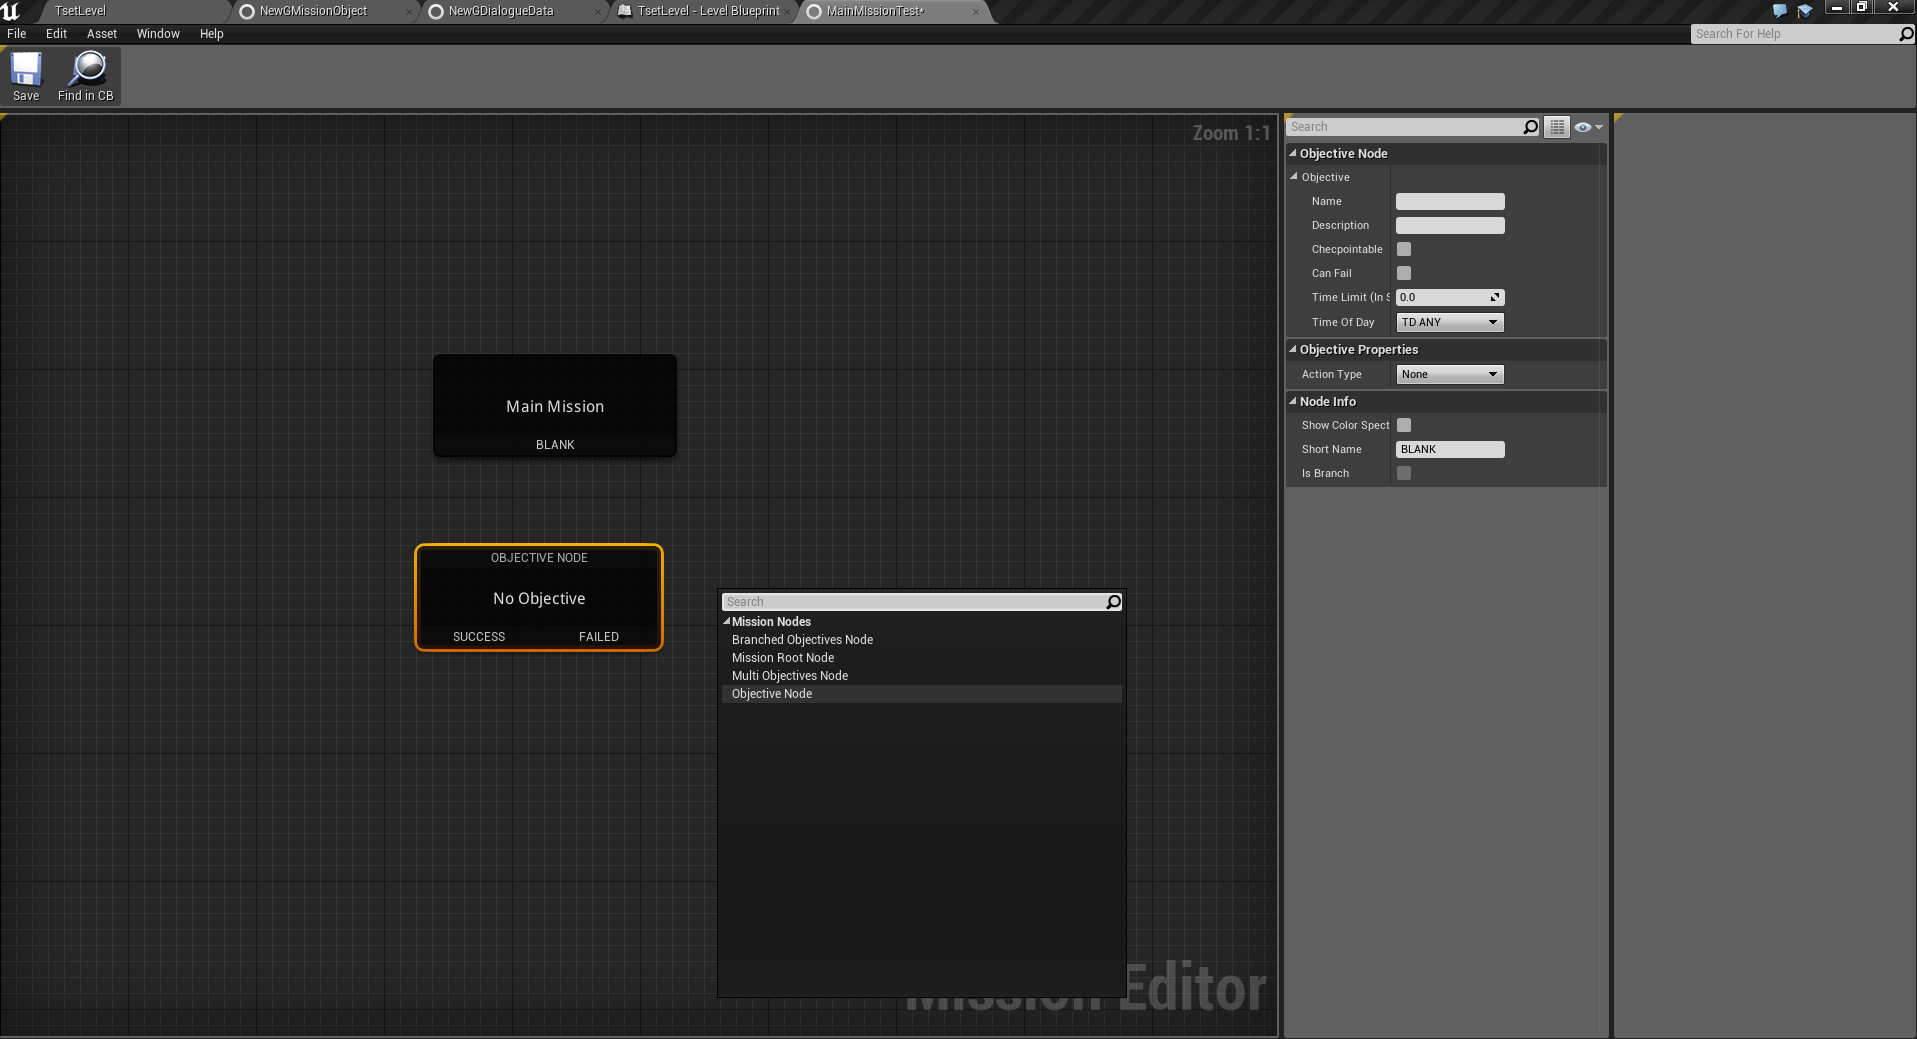
\includegraphics[scale=0.2]{ObjectiveNode.png}
	  \end{center}
	  \begin{center}
	  \textit{OBJECTIVE NODE}\\
	  \----------------------------------
	  \end{center}
	  This is the node where we design our objective.
	   \begin{center}
	  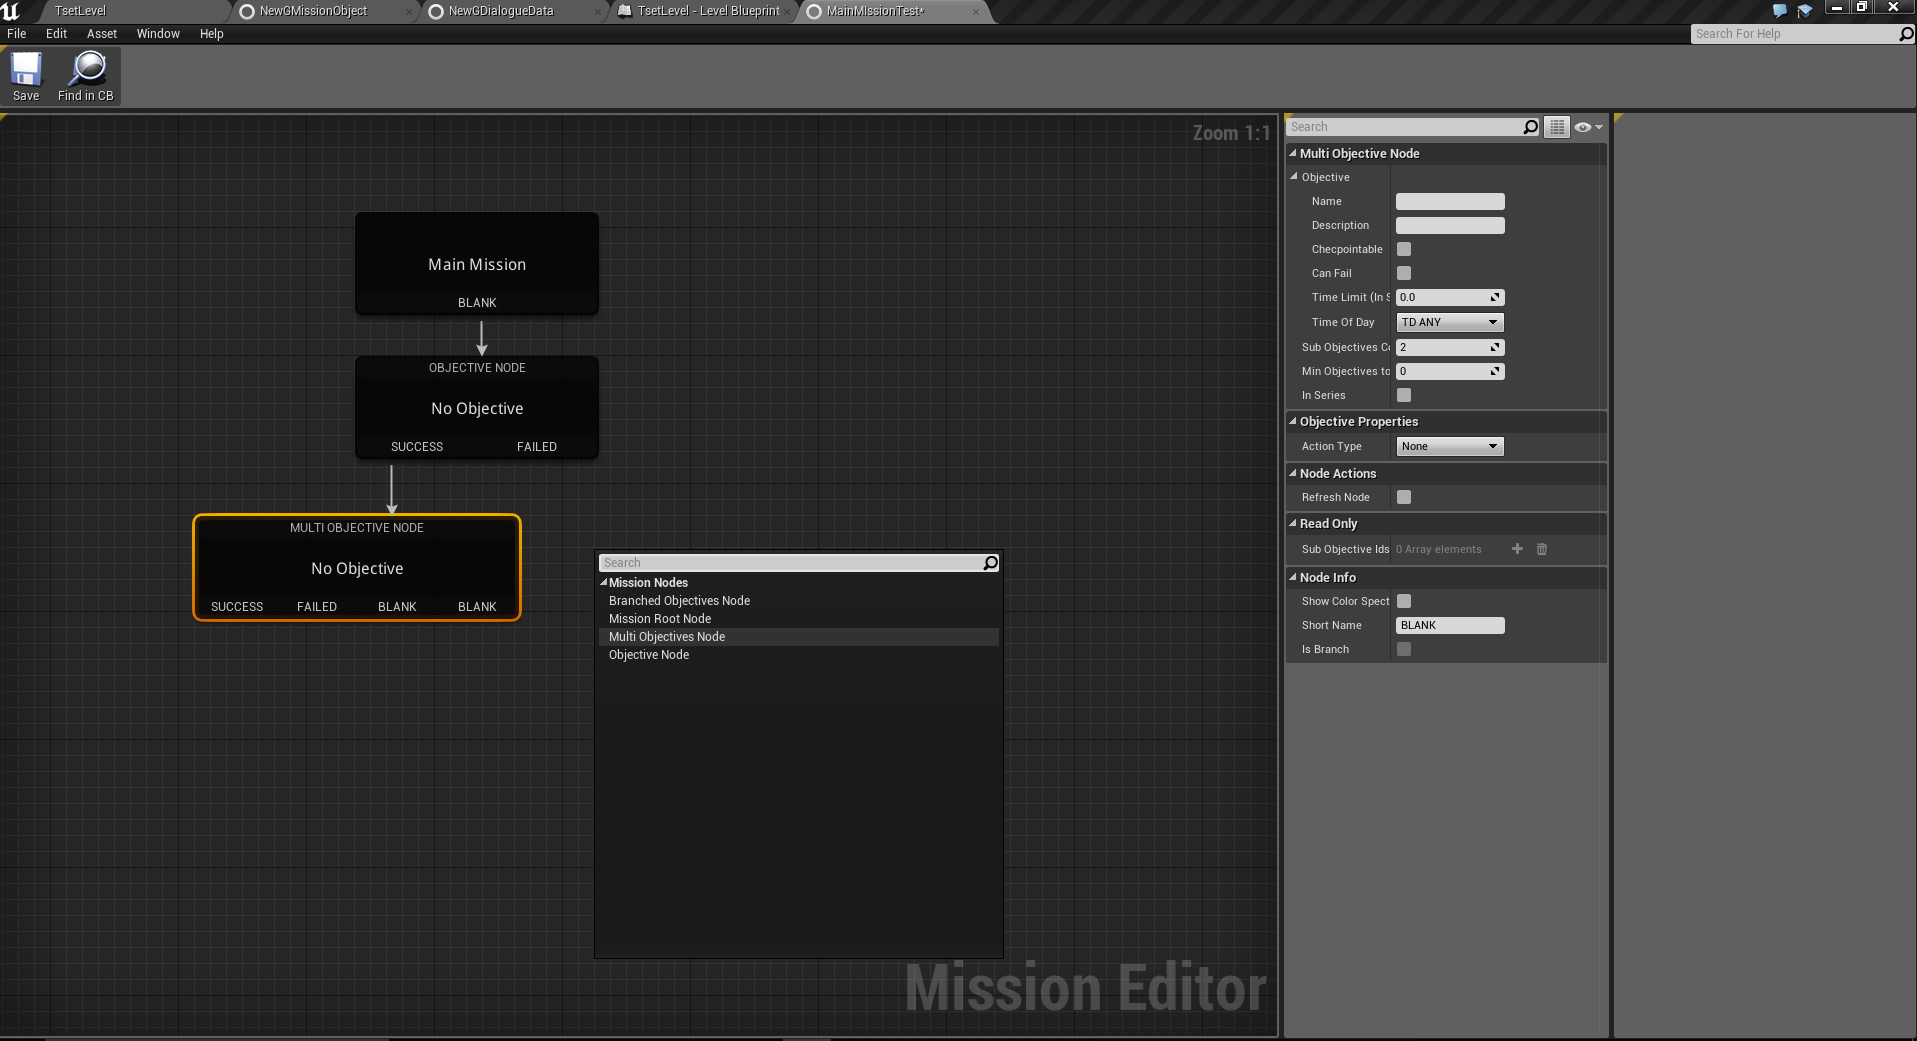
\includegraphics[scale=0.2]{MultiObjectiveNode.png}
	  \end{center}
	  \begin{center}
	  \textit{MULTI OBJECTIVE NODE}\\
	  \----------------------------------
	  \end{center}
	  This node same as an objective node but in this node we can design an objective which can have multiple objective.
	   \begin{center}
	  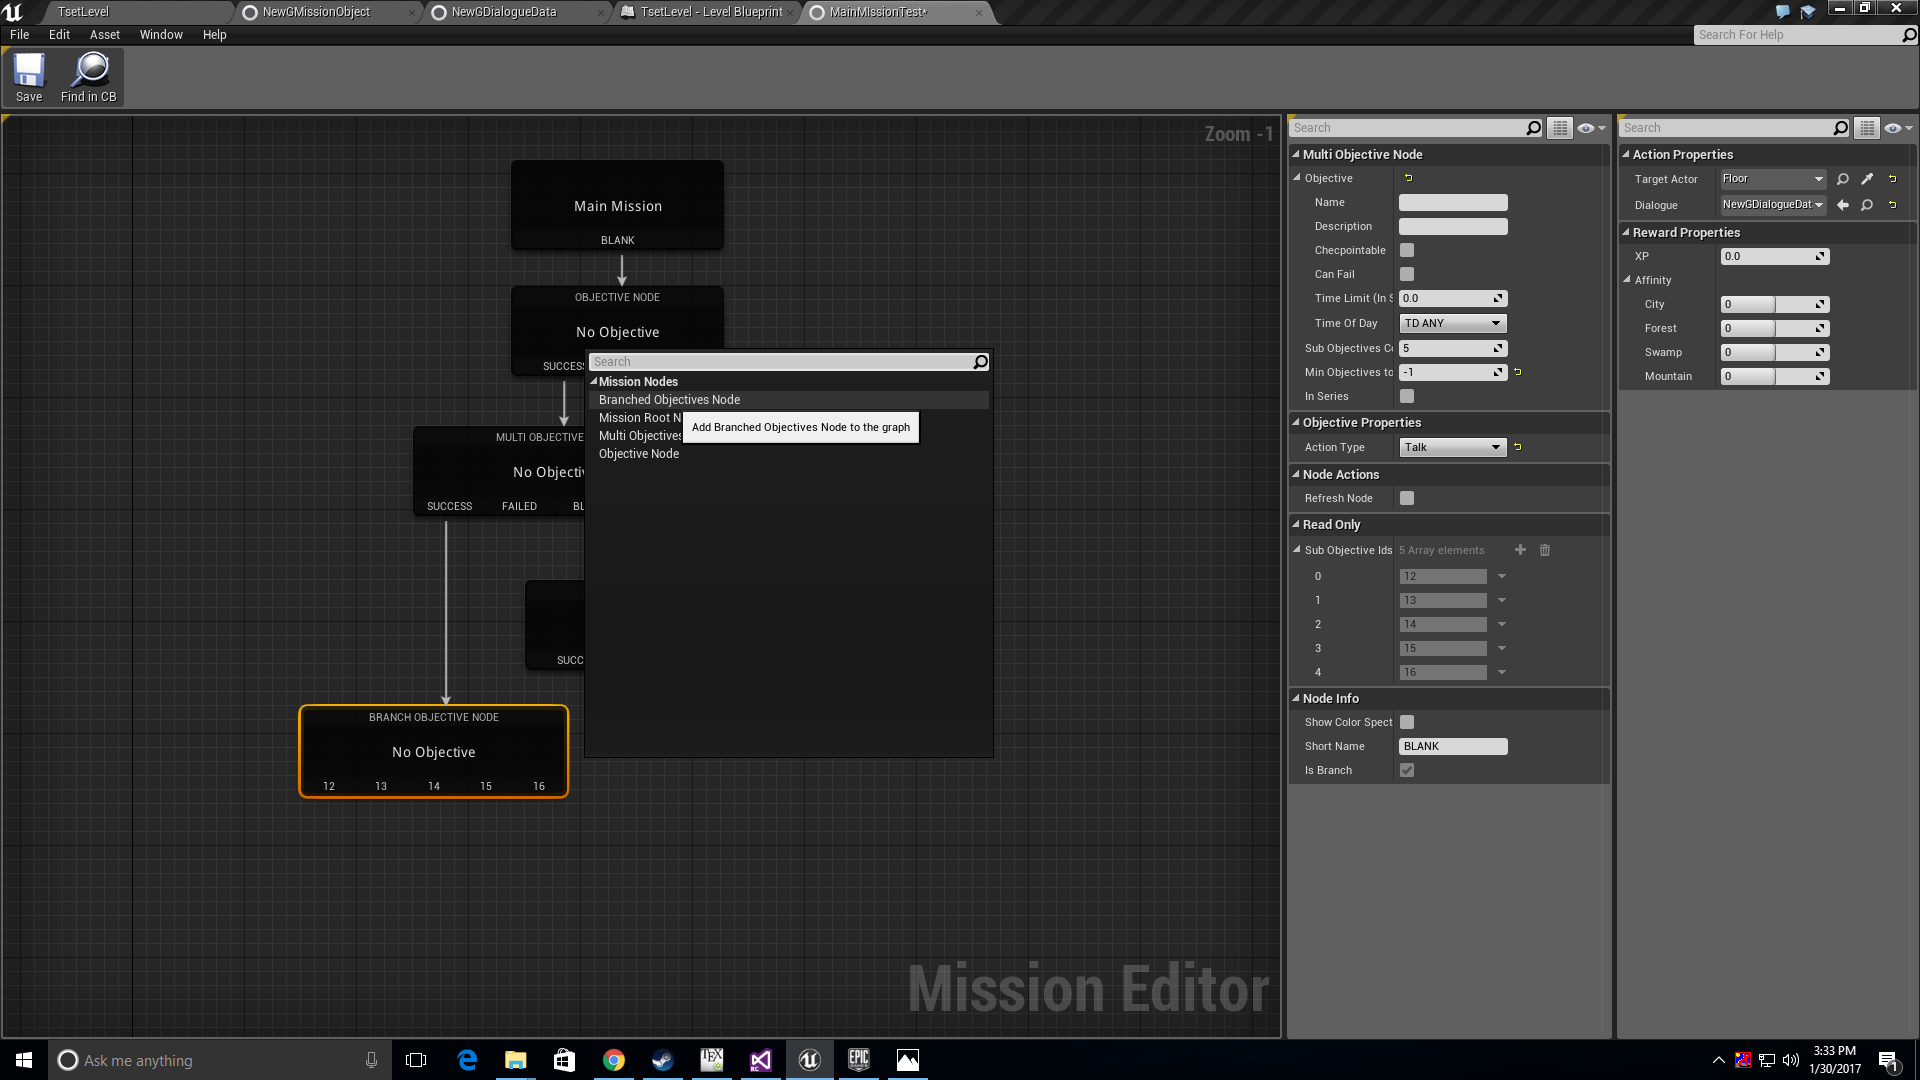
\includegraphics[scale=0.2]{BranchedObjectiveNode.png}
	  \end{center}
	  \begin{center}
	  \textit{BRANCHED OBJECTIVE NODE}\\
	  \----------------------------------------------
	  \end{center}
	  \subsubsection{MISSION ROOT NODE}
	  \subsection{DialogueGraph}
	  \section{Example}
\end{document}